Ce travail de modélisation s'inscrit dans le cadre de l'amélioration de la description du comportement du corium au fond de la cuve pour les besoins d'évaluation d'une stratégie de rétention en cuve (``In vessel retention'' -- IVR) par un refroidissement externe par renoyage du puits de cuve (``External Reactor Vessel Cooling'' -- ERVC) \cite{Theofanous1997, Kymalainen1997}. Dans ce cadre, le risque principal de percement ``thermique'' de la cuve (\textit{i.e.} d'avoir un flux de chaleur suffisamment important pendant suffisamment longtemps pour qu'il y ait assèchement en paroi externe de la cuve et donc perte du refroidissement) est associé à l'existence d'une couche métallique au-dessus du bain de corium en contact direct avec la cuve (sans croûte réfractaire à l'interface). En effet, dans ce cas, la géométrie de la couche (de par un rapport entre surface latérale et surface axiale faible) et la conductivité élevée de cette phase métallique concourent à un phénomène de concentration du flux de chaleur (``focusing effect'') au niveau de la surface latérale de cette couche métal.

Le comportement d'un bain de corium en fond de cuve résulte du couplage entre deux grands types de phénomènes: alors que la thermochimie du bain conditionne sa séparation en plusieurs phases liquides (immiscibles) et solides, son comportement thermohydraulique au travers de la convection naturelle qui s'y installe détermine \textit{in fine} le flux de chaleur à son interface. La \Fig{corium_stratif} montre une vision ``idéalisée'' de la répartition des phases typiques des modélisations mises en \oe{}uvre pour le corium en fond de cuve (il s'agit, en l’occurrence du modèle macroscopique de PROCOR \cite{LeTellier2015}). On y distingue plusieurs phases liquides (une oxyde et plusieurs métalliques) qui, en fonction de leur densité, ont tendance à se stratifier gravitairement ainsi qu'une phase solide (appelée ``croûte'') à la frontière d'une partie de ces ``couches'' liquides. 

\begin{figure}[H]
 \centering
 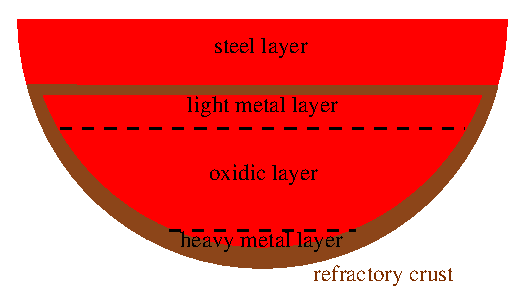
\includegraphics[width=0.5\textwidth]{Figures/multilayer.eps}
 \caption{Représentation idéalisée des phases ségrégées d'un bain de corium dans le modèle de PROCOR}
 \label{fig:corium_stratif}
\end{figure}

L'approche classiquement mise en \oe{}uvre pour évaluer une stratégie IVR s'appuie sur des calculs de thermique en stationnaire pour des configurations postulées des différentes phases en présence. C'est, par exemple, le cas de la démonstration de sûreté du réacteur VVER440 de la centrale de Loviisa \cite{Kymalainen1997} ou encore du réacteur AP1000 en construction de par le monde \cite{Esmaili2004}. Les configurations du bain postulées sont obtenues à partir de considérations vis-à-vis de l'équilibre thermodynamique du système en se plaçant dans des conditions jugées pénalisantes ou ``enveloppes'' vis-à-vis du ``focusing effect''. Une telle approche est limitée par :
\begin{itemize}
 \item le choix de l'inventaire des matériaux fondus mis en présence dans le fond de cuve. En effet, cet inventaire est largement dépendant du déroulement de l'accident (dégradation du c\oe ur et relocalisation en fond de cuve) et le découplage que requiert une telle méthodologie n'est pas toujours justifiable, en particulier, vis-à-vis de la masse d'acier qui dépend directement du transitoire en fond de cuve \cite{Seiler2014} ;
 \item l’exclusion qui est faite de situations transitoires qui peuvent être plus pénalisantes que la configuration stationnaire, en particulier, vis-à-vis de la formation de la couche métallique supérieure responsable du ``focusing effect'' \cite{Rempe1998}.
\end{itemize}

C'est dans l'objectif de pallier aux manques de cette approche que les premières études avec PROCOR sur l'IVR ont été menées à partir de 2013 : une première application PROCOR dédiée au comportement du corium en fond de cuve a été construite et a servi à réaliser des études de sensibilité \cite{LeTellier2014}. Les résultats associés ont permis de préciser les axes principaux de R\&D en ce qui concerne l'amélioration de la modélisation dans l'objectif de réduire conservatisme et incertitudes. Ces axes ont été inscrits dans le projet Européen H2020 IVMR\footnote{\url{https://cordis.europa.eu/project/rcn/196923_fr.html}} (In-Vessel Melt Retention) débuté en 2015, coordonné par l'IRSN et qui s'achèvera en 2019. Dans le cadre de ce projet, un exercice de type ``PIRT'' (Phenomena Identification Ranking Table) \cite{Carenini2019a} ainsi qu'une série de benchmarks portant sur les bains de corium en fond de cuve \cite{Carenini2019} ont été réalisés afin d'identifier plus précisément et de partager de manière consensuelle ces axes de R\&D et le besoin en modélisation associé.\footnote{On notera que ces benchmarks sont dans la continuité des benchmarks initiés entre PROCOR et les versions propriétaires de MAAP4 \cite{maap4} et MAAP5 \cite{maap5} développées par EDF (voir \cite{Bakouta2015}) et repris ensuite avec l'IRSN et le code ASTEC \cite{Carenini2014}.}

Les grands axes d'amélioration (pour la réduction des biais et incertitudes) liés directement à la modélisation du corium en fond de cuve qui se sont dégagés peuvent être classés comme suit \cite{LeTellier2014,Fichot2018} :
\begin{description}
 \item[thermohydraulique d'un bain stratifié] avec en premier lieu, les transferts thermiques relatifs à la couche métallique supérieure et la question des conditions aux limites associées ; c'est l'objet des travaux menés par une approche CFD (``Computational Fluid Dynamics'') dans le cadre du WP2.3 du projet IVMR et de la remontée d'échelle, en vue de l'amélioration des modèles intégraux, réalisée dans le cadre de la fiche ``Modélisation des accidents graves'' du projet CORIU \cite{Peybernes2019} ; 
 \item[cinétique de stratification] avec les transferts de masse inter-couches et les instabilités de Rayleigh-Taylor découlant des changements de densités induits par cette cinétique de ``partitionnement'' des espèces ; c'est l'objet des travaux menés dans le WP3.1 (CORDEB2) et WP3.2 (VITI-CORMET) du projet IVMR \cite{Pivano2019} ainsi que dans la cadre de la fiche ``R\&D en support à la modélisation du corium'' du projet CORIU \cite{LeTellier2018} ;
 \item[croûtes aux interfaces] pour leur influence sur les deux points précédents : résistance thermique si elle se trouve à l'interface entre les phases métalliques du bain de corium et la paroi de la cuve, ``barrière'' aux échanges de masse inter-couches.
\end{description}
C'est à ce dernier point que s'adresse le travail de modélisation rapporté dans cette note et plus particulièrement à la description de la croûte latérale. En effet, dans la version initiale du modèle de bain (telle que présentée dans \cite{LeTellier2014}), cette croûte n'est pas explicitement modélisée et ne joue un rôle que vis-à-vis de la condition en limite thermique des couches liquides. Dans une phase d'inversion de stratification en particulier (\textit{i.e.} lorsque la phase métallique lourde ``remonte'' au dessus de la phase oxyde), ce traitement par une croûte ``fictive'' n'est plus adapté. Par ailleurs, dans ce contexte où, globalement, la modélisation thermochimique mise en \oe{}uvre doit évoluer vers une description plus fine et plus complète des phénomènes \cite{Fichot2015}, la modélisation thermique explicite de cette croûte est un préalable nécessaire. 
\begin{remark}
Notons qu'un autre aspect déterminant de la description du transitoire en fond de cuve est associé à la relocalisation de l'acier fondu dans le bain avec, en particulier, le devenir de l'acier fondu de la paroi de la cuve vis-à-vis des différentes couches du bain. En l'état actuel des connaissances, il n'y a pas de modèle à proprement dit de ce cheminement dans les codes et cela reste de l'ordre de l'hypothèse (e.g. dans PROCOR, cet acier est toujours relocalisé au-dessus du bain ce qui revient à considérer que la croûte latérale est une ``barrière'' imperméable à l'acier fondu de la paroi de la cuve). Progresser sur ce point du point de la modélisation requiert aussi une description explicite de la croûte dans un modèle fond de cuve. Dans un second temps, des modèles concernant la thermochimie (dissolution de la croûte par l'acier liquide) et la thermomécanique devront être étudiés pour évaluer l'hypothèse de relocalisation de l'acier liquide.
\end{remark}
Dans ce contexte, cette note décrit la modélisation explicite de la thermique et de la dynamique de la croûte latérale d'un bain de corium en fond de cuve développée pour la version v2.3 de la plateforme PROCOR. Cette action s'inscrit dans le cadre de la fiche ``plateforme PROCOR'' du projet CORIU pour les années 2017 et 2018. Ce modèle, en phase de tests, sera disponible à l'utilisateur de l'application PROCOR-FDC (dédiée au comportement du corium en fond de cuve d'un réacteur à eau pressurisée) dans sa version 2.3.

Avec ce modèle, on cherche en particulier à s'affranchir des hypothèses de macro-ségrégation du modèle initial de PROCOR qui conduisent à une température uniforme à l'interface des couches du bain entouré de sa croûte réfractaire. Cette modélisation est en effet problématique lors de l'inversion de stratification (formation d'une couche métallique légère au-dessus du bain oxyde) puisqu'elle conduit à considérer que la couche métallique légère se retrouve toujours en face d'une croûte réfractaire.

Cette note s'articule comme suit. La section \ref{sect:modelisation} est consacrée à la description du modèle en tant que tel. Un test numérique de vérification illustrant le comportement du modèle souple est présenté à la section \ref{sect:num}. Et, finalement, conclusions et perspectives sont présentées à la section \ref{sect:conclusion}.
